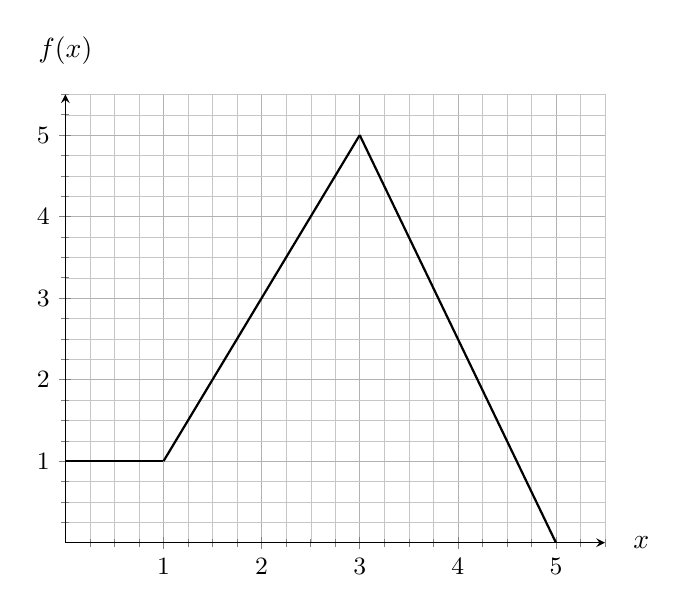
\begin{tikzpicture}
    \begin{axis}[
        grid=both,
        grid style={line width=.1pt, draw=gray!45},
        major grid style={line width=.2pt,draw=gray!60},
        every tick label/.append style={font=\small},
        axis x line = middle,
        axis y line = middle,
            every axis y label/.style={at={(ticklabel cs:1.15)}},
            %ytick = {-4, -2, -3, -1, 1, 2, 3, 4},
        y label style={at={(axis description cs:0,1.15)},anchor=north},
            ylabel = {$f(x)$},
            every axis x label/.style= {at ={(ticklabel cs:1)}},
            %xtick = {-4,-3,-2,-1,1,2,3,4},
            x label style={at={(axis description cs:1.1,0)},anchor=east},
            xlabel = {$x$},
            xmax = 5.5, ymin = 0, ymax = 5.5,
            minor tick num = 3
    ]
    
        \addplot[thick,domain = 0:1] {1};
        \addplot[thick,domain = 1:3] {2*x-1};
        \addplot[thick,domain = 3:5] {-2.5*x+12.5};
    \end{axis}
\end{tikzpicture}